%===================================================================%
\section{Schéma d'Architecture}
%===================================================================%
L'application sera construite d'après le schéma d'architecture suivant :

\begin{figure}[H]
    \centering
    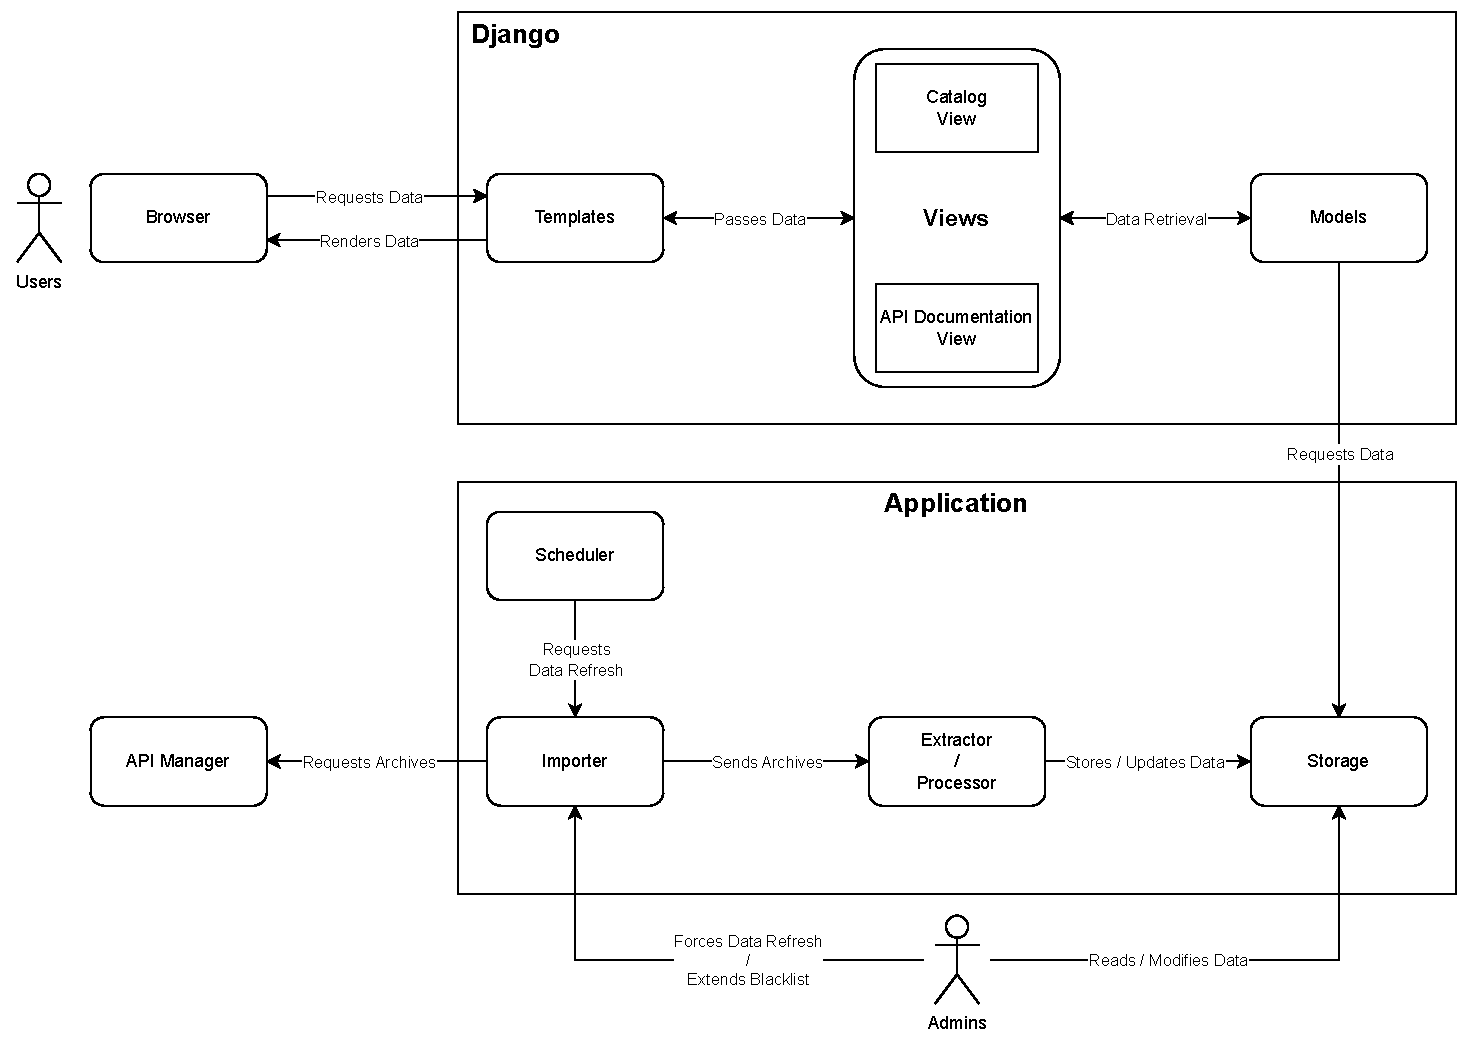
\includegraphics[width=1.00\textwidth]{img/architecture_diagram.pdf}
    \caption{Schéma d'architecture}
\end{figure}

%%%%%%%%%%%%%%%%%%%%%%%%%%%%%%%%%%%%%%%%%%%%%%%%%%%%%%%%%%%%%%%%%%%%%
%                                                                   %
%                                                                   %
%                                                                   %
%                                                                   %
%                                                                   %
%                                                                   %
%                                                                   %
%                                                                   %
%===================================================================%
\section{Technologies \& Frameworks}
%===================================================================%
\begin{itemize}
    \item[$\bullet$] \textbf{Django} : le framework web sera probablement Django car il est déjà connu et utilisé dans le service et permet de lier facilement les URLs aux différentes vues qui seront générées automatiquement en utilisant la fonctionnalité de template de Django.
    \item[$\bullet$] \textbf{Cron} : le planificateur automatique utilisé sera cron car il est déjà connu et fiable. Il permettra de régénérer automatiquement le catalogue des APIs à intervalle régulier.
    \item[$\bullet$] \textbf{Python} : le langage permettra de créer facilement les programmes d'importation et d'extraction d'autant plus que le framework Django est déjà lui-même basé sur ce langage, cela facilitera la maintenance de l'application.
    \item[$\bullet$] \textbf{Docker} : nous isolerons dans des conteneurs docker les composants suivants :
    \begin{itemize}
        \item[$\circ$] le framework Django
        \item[$\circ$] le planificateur automatique cron
        \item[$\circ$] l'application d'importation et d'extraction
    \end{itemize}
\end{itemize}

%%%%%%%%%%%%%%%%%%%%%%%%%%%%%%%%%%%%%%%%%%%%%%%%%%%%%%%%%%%%%%%%%%%%%
%                                                                   %
%                                                                   %
%                                                                   %
%                                                                   %
%                                                                   %
%                                                                   %
%                                                                   %
%                                                                   %
%===================================================================%
% \section{???}
%===================================================================%
% BLABLABLA

%%%%%%%%%%%%%%%%%%%%%%%%%%%%%%%%%%%%%%%%%%%%%%%%%%%%%%%%%%%%%%%%%%%%%